\documentclass{article}

% content/resources/templates/preamble.tex
\usepackage[margin=0.6in]{geometry}
\author{Milav Dabgar}
\usepackage{amsmath,amssymb,amsthm}
\usepackage{booktabs}
\usepackage{multirow}
\usepackage{xcolor}
\usepackage{tcolorbox}
\tcbuselibrary{breakable,skins}
\usepackage[colorlinks=true,linkcolor=blue]{hyperref}
\usepackage{titlesec}
\usepackage{enumitem}
\usepackage{tikz}
\usepackage{pgfplots}
\usepackage{circuitikz}
\usepackage[version=4]{mhchem}
\usepackage{longtable}
\usepackage{array}
\usepackage{float}
\usepackage{caption}
\usepackage{listings}

\lstset{
  basicstyle=\small\ttfamily,
  breaklines=true,
  breakatwhitespace=false,
  postbreak=\mbox{\textcolor{red}{$\hookrightarrow$}\space},
  float=false,
  numbers=left,
  numberstyle=\tiny\color{gray},
  numbersep=10pt,
  xleftmargin=2em,
  keywordstyle=\color{blue},
  commentstyle=\color{green!60!black},
  stringstyle=\color{purple},
  backgroundcolor=\color{gray!5},
  showstringspaces=false,
  tabsize=2,
  captionpos=b,
  keepspaces=true,
  columns=flexible
}

\pgfplotsset{compat=1.18}
\usetikzlibrary{shapes,arrows,positioning,calc,patterns,decorations.pathmorphing,decorations.markings,arrows.meta}

% Color scheme
\definecolor{headcolor}{RGB}{0,102,204}
\definecolor{keycolor}{RGB}{220,20,60}
\definecolor{solutioncolor}{RGB}{34,139,34}
\definecolor{mnemoniccolor}{RGB}{148,0,211}
\definecolor{codecolor}{RGB}{0,0,100}

% Spacing
\setlength{\parskip}{3pt}
\setlist[itemize]{nosep}
\setlist[enumerate]{nosep}

% Title formatting
\titleformat{\section}{\Large\bfseries\color{headcolor}}{\thesection}{1em}{}
\titleformat{\subsection}{\large\bfseries\color{headcolor}}{\thesubsection}{1em}{}

% Pandoc tightlist compatibility
\providecommand{\tightlist}{%
  \setlength{\itemsep}{0pt}\setlength{\parskip}{0pt}}

% Pandoc longtable compatibility
\newcounter{none}
\def\thenone{}


% content/resources/templates/english-boxes.tex

% Custom environments
\newtcolorbox{solutionbox}{
 breakable,
 enhanced,
 colback=solutioncolor!5!white,
 colframe=solutioncolor!75!black,
 fonttitle=\bfseries,
 title=Solution
}

\newtcolorbox{solutionboxnobreak}{
 colback=solutioncolor!5!white,
 colframe=solutioncolor!75!black,
 fonttitle=\bfseries,
 title=Solution
}

\newtcolorbox{keyformula}{
 breakable,
 enhanced,
 colback=keycolor!5!white,
 colframe=keycolor!75!black,
 fonttitle=\bfseries,
 title=Key Formula
}

\newtcolorbox{mnemonicboxenv}{
 breakable,
 enhanced,
 colback=mnemoniccolor!5!white,
 colframe=mnemoniccolor!75!black,
 fonttitle=\bfseries,
 title=Mnemonic
}

\newcommand{\mnemonicbox}[1]{%
  \begin{mnemonicboxenv}
    #1
  \end{mnemonicboxenv}
}


% Custom commands for GTU solutions
% This file defines semantic commands for consistent formatting

% Question command with automatic formatting
\newcommand{\question}[2]{%
  \section*{Question #1}%
  \textbf{#2}%
}

% OR question variant
\newcommand{\questionor}[2]{%
  \section*{Question #1 OR}%
  \textbf{#2}%
}

% Proper table environment with caption
\newenvironment{answertable}[1]{%
  \begin{table}[htbp]
  \centering
  \caption{#1}
}{%
  \end{table}
}

% Proper figure environment for diagrams
\newenvironment{answerdiagram}[1]{%
  \begin{figure}[htbp]
  \centering
  \caption{#1}
}{%
  \end{figure}
}

% Semantic markup for key terms
\newcommand{\keyword}[1]{\textbf{#1}}
\newcommand{\code}[1]{\texttt{#1}}
\newcommand{\classname}[1]{\texttt{#1}}
\newcommand{\methodname}[1]{\texttt{#1}}

% Proper quotation marks
\newcommand{\mnemonic}[1]{``#1''}


\title{Microprocessor \& Microcontroller Systems (1333202) - Winter 2023 Solution}
\date{January 16, 2024}

\begin{document}
\maketitle

\questionmarks{1(a)}{3}{Define Microprocessor.}

\begin{solutionbox}
A microprocessor is a single-chip CPU that contains all the arithmetic, logic, and control circuitry required to perform the functions of a digital computer's central processing unit.

\begin{center}
\captionof{table}{Microprocessor Key Features}
\begin{tabulary}{\linewidth}{|L|L|}
\hline
\textbf{Feature} & \textbf{Description} \\ \hline
\textbf{Single Chip} & Complete CPU on one integrated circuit \\ \hline
\textbf{Processing Unit} & Executes instructions and performs calculations \\ \hline
\textbf{Control Logic} & Manages system operations and data flow \\ \hline
\end{tabulary}
\end{center}

\begin{itemize}
    \item \keyword{Central Processing Unit}: Core component that executes instructions
    \item \keyword{Integrated Circuit}: All functions combined on single silicon chip
    \item \keyword{Programmable Device}: Can execute different programs based on stored instructions
\end{itemize}
\end{solutionbox}

\begin{mnemonicbox}
\mnemonic{Single Chip CPU = Smart Computer Processor Unit}
\end{mnemonicbox}

\questionmarks{1(b)}{4}{Explain Flag register of microprocessor.}

\begin{solutionbox}
The Flag register stores status information about the result of arithmetic and logical operations performed by the ALU.

\begin{center}
\captionof{table}{8085 Flag Register Bits}
\begin{tabulary}{\linewidth}{|L|L|L|}
\hline
\textbf{Flag} & \textbf{Position} & \textbf{Purpose} \\ \hline
\textbf{S (Sign)} & Bit 7 & Indicates sign of result (1=negative, 0=positive) \\ \hline
\textbf{Z (Zero)} & Bit 6 & Set when result is zero \\ \hline
\textbf{AC (Auxiliary Carry)} & Bit 4 & Carry from bit 3 to bit 4 \\ \hline
\textbf{P (Parity)} & Bit 2 & Even parity flag \\ \hline
\textbf{CY (Carry)} & Bit 0 & Carry from MSB \\ \hline
\end{tabulary}
\end{center}

\begin{itemize}
    \item \keyword{Status Indicator}: Shows condition of last operation result
    \item \keyword{Conditional Instructions}: Used for branching and decision making
    \item \keyword{5 Active Flags}: Sign, Zero, Auxiliary Carry, Parity, and Carry flags
\end{itemize}
\end{solutionbox}

\begin{mnemonicbox}
\mnemonic{Flags Show Zero, Sign, Parity, Auxiliary, Carry}
\end{mnemonicbox}

\questionmarks{1(c)}{7}{Explain format of instruction of microprocessor with example.}

\begin{solutionbox}
Microprocessor instructions consist of opcode and operand fields that specify the operation and data locations.

\begin{center}
\captionof{table}{8085 Instruction Format Types}
\begin{tabulary}{\linewidth}{|L|L|L|L|}
\hline
\textbf{Format} & \textbf{Size} & \textbf{Structure} & \textbf{Example} \\ \hline
\textbf{1-Byte} & 8 bits & Opcode only & \code{MOV A,B} \\ \hline
\textbf{2-Byte} & 16 bits & Opcode + 8-bit data & \code{MVI A,05H} \\ \hline
\textbf{3-Byte} & 24 bits & Opcode + 16-bit address & \code{LDA 2000H} \\ \hline
\end{tabulary}
\end{center}

\begin{center}
\begin{tikzpicture}[node distance=1.5cm, auto]
    \node [gtu block] (IF) {Instruction Format};
    \node [gtu block, below left=1cm and 0.5cm of IF] (Opcode) {Opcode Field};
    \node [gtu block, below right=1cm and 0.5cm of IF] (Operand) {Operand Field};
    
    \node [gtu state, below=1cm of Opcode, align=center] (OC) {Operation Code\\Specifies Operation};
    \node [gtu state, below=1cm of Operand, align=center] (OD) {Data/Address\\Specifies Source/Destination};
    
    \path [gtu arrow] (IF) -- (Opcode);
    \path [gtu arrow] (IF) -- (Operand);
    \path [gtu arrow] (Opcode) -- (OC);
    \path [gtu arrow] (Operand) -- (OD);
\end{tikzpicture}
\captionof{figure}{Instruction Format Structure}
\end{center}

\begin{itemize}
    \item \keyword{Opcode Field}: Defines the operation to be performed (ADD, MOV, JMP)
    \item \keyword{Operand Field}: Contains data, register, or memory address information
    \item \keyword{Variable Length}: Instructions can be 1, 2, or 3 bytes long
    \item \keyword{Addressing Modes}: Different ways to specify operand location
\end{itemize}
\end{solutionbox}

\begin{mnemonicbox}
\mnemonic{Opcode Operations + Operand Objects = Complete Commands}
\end{mnemonicbox}

\questionmarks{1(c OR)}{7}{Explain function of ALU, Control Unit and CPU of Microprocessor.}

\begin{solutionbox}
The CPU consists of three main functional units that work together to execute instructions.

\begin{center}
\captionof{table}{CPU Components and Functions}
\begin{tabulary}{\linewidth}{|L|L|L|}
\hline
\textbf{Component} & \textbf{Primary Function} & \textbf{Key Operations} \\ \hline
\textbf{ALU} & Arithmetic \& Logic Operations & ADD, SUB, AND, OR, XOR \\ \hline
\textbf{Control Unit} & Instruction Control & Fetch, Decode, Execute \\ \hline
\textbf{CPU} & Overall Processing & Coordinate all operations \\ \hline
\end{tabulary}
\end{center}

\begin{center}
\begin{tikzpicture}[node distance=1.5cm, auto]
    \node [gtu block] (CPU) {CPU};
    \node [gtu block, below left=1.5cm and -0.5cm of CPU, align=center] (ALU) {ALU\\Arithmetic Logic Unit};
    \node [gtu block, below=1.5cm of CPU] (CU) {Control Unit};
    \node [gtu block, below right=1.5cm and -0.5cm of CPU] (RA) {Register Array};
    
    \node [gtu state, below=1cm of ALU, align=center] (Math) {Math Operations\\Logic Operations};
    \node [gtu state, below=1cm of CU, align=center] (IC) {Instruction Control\\Signal Generation};

    \path [gtu arrow] (CPU) -- (ALU);
    \path [gtu arrow] (CPU) -- (CU);
    \path [gtu arrow] (CPU) -- (RA);
    \path [gtu arrow] (ALU) -- (Math);
    \path [gtu arrow] (CU) -- (IC);
\end{tikzpicture}
\captionof{figure}{CPU Components}
\end{center}

\begin{itemize}
    \item \keyword{ALU Functions}: Performs all arithmetic calculations and logical operations
    \item \keyword{Control Unit Tasks}: Manages instruction execution cycle and generates control signals
    \item \keyword{CPU Coordination}: Integrates ALU and Control Unit for complete processing
\end{itemize}
\end{solutionbox}

\begin{mnemonicbox}
\mnemonic{ALU Adds, Control Commands, CPU Coordinates}
\end{mnemonicbox}

\questionmarks{2(a)}{3}{Explain function of ALE signal with diagram.}

\begin{solutionbox}
ALE (Address Latch Enable) signal is used to demultiplex the lower-order address and data lines.

\begin{center}
\captionof{table}{ALE Signal Functions}
\begin{tabulary}{\linewidth}{|L|L|}
\hline
\textbf{Function} & \textbf{Description} \\ \hline
\textbf{Address Latching} & Captures lower 8-bit address \\ \hline
\textbf{Demultiplexing} & Separates address from data \\ \hline
\textbf{Timing Control} & Provides timing reference \\ \hline
\end{tabulary}
\end{center}

\begin{center}
\begin{tikzpicture}[node distance=2cm, auto]
    \node [gtu block, minimum width=2cm, minimum height=2cm] (8085) {8085};
    \node [gtu block, right=3cm of 8085, minimum width=2cm, minimum height=2cm] (Latch) {Latch\\74373};
    
    \draw [->, thick] ([yshift=0.5cm]8085.east) -- node[above] {ALE} ([yshift=0.5cm]Latch.west);
    \draw [<->, thick] ([yshift=-0.5cm]8085.east) -- node[above] {AD0-AD7} ([yshift=-0.5cm]Latch.west);
    
    \draw [->, thick] (Latch.south) -- ++(0,-1) node[below] {A0-A7 (Address)};
\end{tikzpicture}
\captionof{figure}{ALE and Demultiplexing}
\end{center}

\begin{itemize}
    \item \keyword{Active High Signal}: ALE goes high during T1 state
    \item \keyword{External Latching}: Used with 74373 latch to hold address
    \item \keyword{System Timing}: Provides reference for external devices
\end{itemize}
\end{solutionbox}

\begin{mnemonicbox}
\mnemonic{ALE Always Latches External Addresses}
\end{mnemonicbox}

\questionmarks{2(b)}{4}{Compare microprocessor and microcontroller}

\begin{solutionbox}
\begin{center}
\captionof{table}{Microprocessor vs Microcontroller Comparison}
\begin{tabulary}{\linewidth}{|L|L|L|}
\hline
\textbf{Parameter} & \textbf{Microprocessor} & \textbf{Microcontroller} \\ \hline
\textbf{Design} & General purpose & Application specific \\ \hline
\textbf{Memory} & External RAM/ROM & Internal RAM/ROM \\ \hline
\textbf{I/O Ports} & External interface & Built-in I/O ports \\ \hline
\textbf{Timers} & External & Built-in timers \\ \hline
\textbf{Cost} & Higher system cost & Lower system cost \\ \hline
\textbf{Power} & Higher consumption & Lower consumption \\ \hline
\end{tabulary}
\end{center}

\begin{itemize}
    \item \keyword{Integration Level}: Microcontroller has more integrated components
    \item \keyword{Application Focus}: Microprocessor for computing, microcontroller for control
    \item \keyword{System Complexity}: Microprocessor needs more external components
    \item \keyword{Design Flexibility}: Microprocessor offers more expandability
\end{itemize}
\end{solutionbox}

\begin{mnemonicbox}
\mnemonic{Microprocessor = More Power, Microcontroller = More Control}
\end{mnemonicbox}

\questionmarks{2(c)}{7}{Draw \& explain block diagram of microprocessor.}

\begin{solutionbox}
The 8085 microprocessor consists of several functional blocks that work together.

\begin{center}
\begin{tikzpicture}[node distance=1.5cm, auto]
    \node [gtu block] (ALU) {ALU};
    \node [gtu block, left=of ALU] (ACC) {Accumulator};
    \node [gtu block, above=of ALU] (TMP) {Temp Reg};
    \node [gtu block, right=of ALU] (FLAG) {Flags};
    
    \node [gtu block, below=2cm of ALU] (ID) {Instruction Decoder};
    \node [gtu block, left=of ID] (IR) {Instruction Reg};
    \node [gtu block, right=of ID] (TC) {Timing \& Control};
    
    \node [gtu block, below=2cm of ID] (AB) {Address Buffer};
    \node [gtu block, right=of AB] (ADB) {Address/Data Buffer};
    
    \node [gtu block, left=of AB, align=center] (Regs) {Register Array\\B,C,D,E,H,L\\PC, SP};

    % Connections (Simplified)
    \path [gtu arrow] (ACC) -- (ALU);
    \path [gtu arrow] (TMP) -- (ALU);
    \path [gtu arrow] (ALU) -- (FLAG);
    \path [gtu arrow] (IR) -- (ID);
    \path [gtu arrow] (ID) -- (TC);
\end{tikzpicture}
\captionof{figure}{8085 Architecture Block Diagram}
\end{center}

\begin{center}
\captionof{table}{Block Functions}
\begin{tabulary}{\linewidth}{|L|L|}
\hline
\textbf{Block} & \textbf{Function} \\ \hline
\textbf{ALU} & Arithmetic and logical operations \\ \hline
\textbf{Register Array} & Temporary data storage (B,C,D,E,H,L) \\ \hline
\textbf{Control Unit} & Instruction execution control \\ \hline
\textbf{Address Buffer} & Drive address bus lines \\ \hline
\end{tabulary}
\end{center}

\begin{itemize}
    \item \keyword{Data Path}: Information flows between registers through internal bus
    \item \keyword{Control Signals}: Generated by timing and control unit
    \item \keyword{Bus Interface}: Connects to external memory and I/O devices
    \item \keyword{Register Operations}: Temporary storage for operands and results
\end{itemize}
\end{solutionbox}

\begin{mnemonicbox}
\mnemonic{Blocks Build Better Processing Systems}
\end{mnemonicbox}

\questionmarks{2(a OR)}{3}{Explain 16 bits registers of microprocessor.}

\begin{solutionbox}
The 8085 has three 16-bit registers formed by combining 8-bit register pairs.

\begin{center}
\captionof{table}{16-bit Registers}
\begin{tabulary}{\linewidth}{|L|L|L|}
\hline
\textbf{Register} & \textbf{Formation} & \textbf{Purpose} \\ \hline
\textbf{PC} & Single 16-bit & Program Counter - next instruction address \\ \hline
\textbf{SP} & Single 16-bit & Stack Pointer - top of stack address \\ \hline
\textbf{HL} & H + L registers & Memory pointer - data address \\ \hline
\end{tabulary}
\end{center}

\begin{itemize}
    \item \keyword{Program Counter}: Automatically increments to next instruction
    \item \keyword{Stack Pointer}: Points to last pushed data on stack
    \item \keyword{HL Pair}: Most frequently used for memory addressing
\end{itemize}
\end{solutionbox}

\begin{mnemonicbox}
\mnemonic{PC Points Program, SP Stacks Properly, HL Holds Location}
\end{mnemonicbox}

\questionmarks{2(b OR)}{4}{Explain de-multiplexing lower order address and data lines with diagram of microprocessor.}

\begin{solutionbox}
The 8085 multiplexes lower 8-bit address with data lines to reduce pin count.

\begin{center}
\captionof{table}{Multiplexed Lines}
\begin{tabulary}{\linewidth}{|L|L|L|}
\hline
\textbf{Lines} & \textbf{T1 State} & \textbf{T2-T4 States} \\ \hline
\textbf{AD0-AD7} & Lower Address A0-A7 & Data D0-D7 \\ \hline
\textbf{ALE Signal} & High & Low \\ \hline
\end{tabulary}
\end{center}

\begin{center}
\begin{tikzpicture}[node distance=2cm, auto]
    \node [gtu block, minimum width=2.5cm, minimum height=2cm] (8085) {8085};
    \node [gtu block, right=4cm of 8085, minimum width=2cm, minimum height=2cm] (Latch) {74373 Latch};
    
    \draw [->, thick] ([yshift=0.5cm]8085.east) -- node[above] {ALE} ([yshift=0.5cm]Latch.west);
    \draw [->, thick] ([yshift=-0.5cm]8085.east) -- node[above, near start] {AD0-AD7} ([yshift=-0.5cm]Latch.west);
    
    \draw [->, thick] (Latch.south) -- ++(0,-1) node[below] {A0-A7 (Address Bus)};
    \draw [->, thick] ([xshift=1.5cm, yshift=-0.5cm]8085.east) -- ++(0,-2.5) node[below] {D0-D7 (Data Bus)};
\end{tikzpicture}
\captionof{figure}{De-multiplexing Circuit}
\end{center}

\begin{itemize}
    \item \keyword{Time Division}: Same lines carry address then data
    \item \keyword{External Latch}: 74373 captures address when ALE is high
    \item \keyword{Signal Separation}: Creates separate address and data buses
\end{itemize}
\end{solutionbox}

\begin{mnemonicbox}
\mnemonic{ALE Always Latches External Address Elegantly}
\end{mnemonicbox}

\questionmarks{2(c OR)}{7}{Draw and explain pin diagram of 8085.}

\begin{solutionbox}
The 8085 is a 40-pin microprocessor with multiplexed address/data bus.

\begin{center}
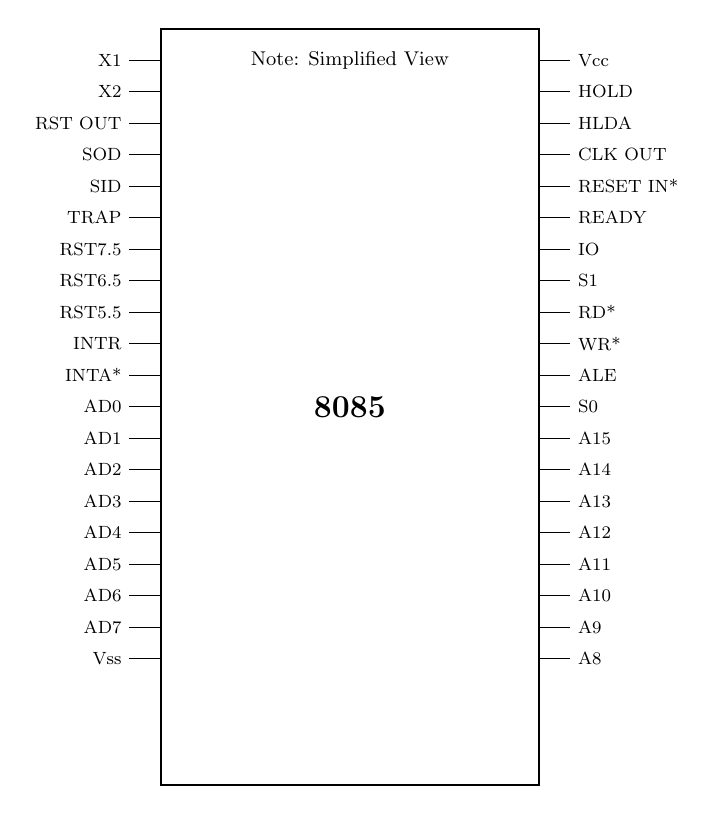
\begin{tikzpicture}[scale=0.8, transform shape]
    % IC Package
    \draw [thick] (0,0) rectangle (6,12);
    \node at (3,6) {\Large \textbf{8085}};
    \node at (3,11.5) {\small Note: Simplified View};
    
    % Left Pins
    \foreach \y/\label in {11.5/X1, 11/X2, 10.5/RST OUT, 10/SOD, 9.5/SID, 9/TRAP, 8.5/RST7.5, 8/RST6.5, 7.5/RST5.5, 7/INTR, 6.5/INTA*, 6/AD0, 5.5/AD1, 5/AD2, 4.5/AD3, 4/AD4, 3.5/AD5, 3/AD6, 2.5/AD7, 2/Vss} {
        \draw (0,\y) -- (-0.5,\y) node[left] {\footnotesize \label};
    }
    
    % Right Pins
    \foreach \y/\label in {11.5/Vcc, 11/HOLD, 10.5/HLDA, 10/CLK OUT, 9.5/RESET IN*, 9/READY, 8.5/IO/M*, 8/S1, 7.5/RD*, 7/WR*, 6.5/ALE, 6/S0, 5.5/A15, 5/A14, 4.5/A13, 4/A12, 3.5/A11, 3/A10, 2.5/A9, 2/A8} {
        \draw (6,\y) -- (6.5,\y) node[right] {\footnotesize \label};
    }
\end{tikzpicture}
\captionof{figure}{8085 Pin Diagram}
\end{center}

\begin{center}
\captionof{table}{Pin Groups}
\begin{tabulary}{\linewidth}{|L|L|L|}
\hline
\textbf{Group} & \textbf{Pins} & \textbf{Function} \\ \hline
\textbf{Address/Data} & AD0-AD7, A8-A15 & Memory addressing and data transfer \\ \hline
\textbf{Control} & ALE, RD*, WR*, IO/M* & Bus control signals \\ \hline
\textbf{Interrupts} & INTR, RST7-RST5, TRAP & Interrupt handling \\ \hline
\textbf{Power} & Vcc, Vss & Power supply connections \\ \hline
\end{tabulary}
\end{center}

\begin{itemize}
    \item \keyword{Multiplexed Bus}: AD0-AD7 carry both address and data
    \item \keyword{Active Low Signals}: Signals with * are active low
    \item \keyword{Crystal Connections}: X1, X2 for clock generation
\end{itemize}
\end{solutionbox}

\begin{mnemonicbox}
\mnemonic{Forty Pins Provide Perfect Processing Power}
\end{mnemonicbox}

\questionmarks{3(a)}{3}{Draw clock and reset circuit of microcontroller}

\begin{solutionbox}
The 8051 requires external clock and reset circuits for proper operation.

\begin{center}
\begin{tikzpicture}[auto, node distance=2cm]
    % Clock Circuit
    \node [gtu block] (8051) {8051};
    \coordinate (XTAL1) at ([yshift=0.5cm]8051.west);
    \coordinate (XTAL2) at ([yshift=-0.5cm]8051.west);
    
    \node [draw, rectangle, left=1.5cm of 8051] (XTAL) {Crystal};
    \draw (XTAL1) -- (XTAL.north east);
    \draw (XTAL2) -- (XTAL.south east);
    
    % Capacitors
    \draw (XTAL.north west) -- ++(-0.5,0) coordinate (C1top);
    \draw (XTAL.south west) -- ++(-0.5,0) coordinate (C2top);
    \draw (C1top) to[capacitor] ++(0,-1) node[ground]{};
    \draw (C2top) to[capacitor] ++(0,-1) node[ground]{};
    
    % Reset Circuit (Conceptual)
    \coordinate (RST) at (8051.north);
    \draw (RST) -- ++(0,1) coordinate (RSTtop);
    \draw (RSTtop) to[R] ++(0,1.5) node[vcc]{+5V};
    \draw (RSTtop) to[C] ++(2,0) node[ground]{};
\end{tikzpicture}
\captionof{figure}{Clock and Reset Circuits}
\end{center}

\begin{center}
\captionof{table}{Circuit Components}
\begin{tabulary}{\linewidth}{|L|L|L|}
\hline
\textbf{Component} & \textbf{Value} & \textbf{Purpose} \\ \hline
\textbf{Crystal} & 11.0592 MHz & Clock generation \\ \hline
\textbf{Capacitors} & 30pF each & Crystal stabilization \\ \hline
\textbf{Reset Resistor} & 10K$\Omega$ & Pull-up for reset \\ \hline
\textbf{Reset Capacitor} & 10$\mu$F & Power-on reset delay \\ \hline
\end{tabulary}
\end{center}

\begin{itemize}
    \item \keyword{Clock Frequency}: Commonly 11.0592 MHz for serial communication
    \item \keyword{Reset Duration}: Must be high for at least 2 machine cycles
    \item \keyword{Power-on Reset}: Automatic reset when power is applied
\end{itemize}
\end{solutionbox}

\begin{mnemonicbox}
\mnemonic{Crystals Create Clock, Resistors Reset Reliably}
\end{mnemonicbox}

\questionmarks{3(b)}{4}{Explain internal RAM of 8051.}

\begin{solutionbox}
The 8051 contains 256 bytes of internal RAM organized in different sections.

\begin{center}
\captionof{table}{Internal RAM Organization}
\begin{tabulary}{\linewidth}{|L|L|L|}
\hline
\textbf{Address Range} & \textbf{Size} & \textbf{Purpose} \\ \hline
\textbf{00H-1FH} & 32 bytes & Register Banks (4 banks $\times$ 8 registers) \\ \hline
\textbf{20H-2FH} & 16 bytes & Bit-addressable area \\ \hline
\textbf{30H-7FH} & 80 bytes & General purpose RAM \\ \hline
\textbf{80H-FFH} & 128 bytes & Special Function Registers (SFRs) \\ \hline
\end{tabulary}
\end{center}

\begin{center}
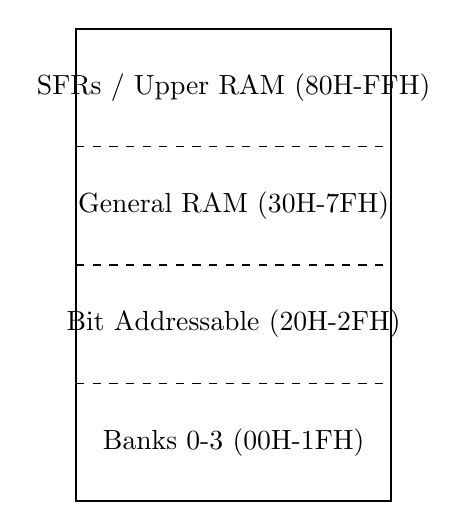
\begin{tikzpicture}
    \draw [thick] (0,0) rectangle (4,6);
    \draw [dashed] (0,1.5) -- (4,1.5);
    \draw [dashed] (0,3) -- (4,3);
    \draw [dashed] (0,4.5) -- (4,4.5);
    
    \node at (2, 0.75) {Banks 0-3 (00H-1FH)};
    \node at (2, 2.25) {Bit Addressable (20H-2FH)};
    \node at (2, 3.75) {General RAM (30H-7FH)};
    \node at (2, 5.25) {SFRs / Upper RAM (80H-FFH)};
\end{tikzpicture}
\captionof{figure}{Internal RAM Map}
\end{center}

\begin{itemize}
    \item \keyword{Register Banks}: Four banks of 8 registers each (R0-R7)
    \item \keyword{Bit Addressing}: Individual bits can be addressed in 20H-2FH area
    \item \keyword{Stack Area}: Usually located in general purpose RAM area
    \item \keyword{Direct Access}: All locations accessible through direct addressing
\end{itemize}
\end{solutionbox}

\begin{mnemonicbox}
\mnemonic{RAM Registers, Bits, General, Special Functions}
\end{mnemonicbox}

\questionmarks{3(c)}{7}{Explain block diagram of 8051.}

\begin{solutionbox}
The 8051 microcontroller integrates CPU, memory, and I/O on a single chip.

\begin{center}
\begin{tikzpicture}[node distance=1.5cm, auto]
    \node [gtu block] (CPU) {CPU Core};
    \node [gtu block, below left=of CPU] (ROM) {4KB ROM};
    \node [gtu block, below right=of CPU] (RAM) {256B RAM};
    \node [gtu block, right=of CPU] (IO) {I/O Ports};
    \node [gtu block, left=of CPU] (Timer) {Timers/Counters};
    \node [gtu block, above=of CPU] (Serial) {Serial Port};
    
    \path [gtu arrow] (CPU) -- (ROM);
    \path [gtu arrow] (CPU) -- (RAM);
    \path [gtu arrow] (CPU) -- (IO);
    \path [gtu arrow] (CPU) -- (Timer);
    \path [gtu arrow] (CPU) -- (Serial);
\end{tikzpicture}
\captionof{figure}{8051 Block Diagram}
\end{center}

\begin{center}
\captionof{table}{Major Blocks}
\begin{tabulary}{\linewidth}{|L|L|}
\hline
\textbf{Block} & \textbf{Function} \\ \hline
\textbf{CPU} & Instruction execution and control \\ \hline
\textbf{Memory} & 4KB ROM + 256B RAM \\ \hline
\textbf{Timers} & Two 16-bit timer/counters \\ \hline
\textbf{I/O Ports} & Four 8-bit bidirectional ports \\ \hline
\textbf{Serial Port} & Full-duplex UART \\ \hline
\textbf{Interrupts} & 5-source interrupt system \\ \hline
\end{tabulary}
\end{center}

\begin{itemize}
    \item \keyword{Harvard Architecture}: Separate program and data memory spaces
    \item \keyword{Built-in Peripherals}: Timers, serial port, interrupts integrated
    \item \keyword{Expandable}: External memory and I/O can be added
    \item \keyword{Control Applications}: Optimized for embedded control tasks
\end{itemize}
\end{solutionbox}

\begin{mnemonicbox}
\mnemonic{Complete Control Chip Contains CPU, Memory, I/O}
\end{mnemonicbox}

\questionmarks{3(a OR)}{3}{Explain function of DPTR and PC.}

\begin{solutionbox}
DPTR and PC are important 16-bit registers in 8051 for memory addressing.

\begin{center}
\captionof{table}{DPTR and PC Functions}
\begin{tabulary}{\linewidth}{|L|L|L|}
\hline
\textbf{Register} & \textbf{Full Form} & \textbf{Function} \\ \hline
\textbf{DPTR} & Data Pointer & Points to external data memory \\ \hline
\textbf{PC} & Program Counter & Points to next instruction address \\ \hline
\end{tabulary}
\end{center}

\begin{itemize}
    \item \keyword{DPTR Usage}: Accessing external RAM and lookup tables
    \item \keyword{PC Function}: Automatically increments after instruction fetch
    \item \keyword{16-bit Addressing}: Both can address 64KB memory space
\end{itemize}
\end{solutionbox}

\begin{mnemonicbox}
\mnemonic{DPTR Data Pointer, PC Program Counter}
\end{mnemonicbox}

\questionmarks{3(b OR)}{4}{Explain different timer modes of microcontroller.}

\begin{solutionbox}
The 8051 has two timers with four different operating modes.

\begin{center}
\captionof{table}{Timer Modes}
\begin{tabulary}{\linewidth}{|L|L|L|}
\hline
\textbf{Mode} & \textbf{Configuration} & \textbf{Purpose} \\ \hline
\textbf{Mode 0} & 13-bit timer & Compatible with 8048 \\ \hline
\textbf{Mode 1} & 16-bit timer & Maximum count capability \\ \hline
\textbf{Mode 2} & 8-bit auto-reload & Constant time intervals \\ \hline
\textbf{Mode 3} & Two 8-bit timers & Timer 0 split operation \\ \hline
\end{tabulary}
\end{center}

\begin{itemize}
    \item \keyword{Mode Selection}: Controlled by TMOD register bits
    \item \keyword{Timer 0/1}: Both timers support modes 0, 1, 2
    \item \keyword{Mode 3 Special}: Only Timer 0 can operate in mode 3
    \item \keyword{Applications}: Delays, baud rate generation, event counting
\end{itemize}
\end{solutionbox}

\begin{mnemonicbox}
\mnemonic{Modes Make Timers Tremendously Versatile}
\end{mnemonicbox}

\questionmarks{3(c OR)}{7}{Explain interrupts of microcontroller.}

\begin{solutionbox}
The 8051 has a 5-source interrupt system for handling external events.

\begin{center}
\captionof{table}{8051 Interrupt Sources}
\begin{tabulary}{\linewidth}{|L|L|L|L|}
\hline
\textbf{Interrupt} & \textbf{Vector Address} & \textbf{Priority} & \textbf{Trigger} \\ \hline
\textbf{Reset} & 0000H & Highest & Power-on/External \\ \hline
\textbf{External 0} & 0003H & High & INT0 pin \\ \hline
\textbf{Timer 0} & 000BH & Medium & Timer 0 overflow \\ \hline
\textbf{External 1} & 0013H & Medium & INT1 pin \\ \hline
\textbf{Timer 1} & 001BH & Low & Timer 1 overflow \\ \hline
\textbf{Serial} & 0023H & Lowest & Serial communication \\ \hline
\end{tabulary}
\end{center}

\begin{center}
\begin{tikzpicture}[node distance=1.5cm, auto]
    \node [gtu block] (IS) {Interrupt System};
    \node [gtu block, below left=of IS] (INT0) {External INT0};
    \node [gtu block, below=of IS] (T0) {Timer 0};
    \node [gtu block, below right=of IS] (INT1) {External INT1};
    \node [gtu block, right=of IS] (Control) {Control Registers\\IE, IP};
    
    \path [gtu arrow] (IS) -- (INT0);
    \path [gtu arrow] (IS) -- (T0);
    \path [gtu arrow] (IS) -- (INT1);
    \path [gtu arrow] (IS) -- (Control);
\end{tikzpicture}
\captionof{figure}{Interrupt System Structure}
\end{center}

\begin{itemize}
    \item \keyword{Interrupt Enable}: IE register controls individual interrupt enables
    \item \keyword{Priority Control}: IP register sets interrupt priorities
    \item \keyword{Vector Addresses}: Each interrupt has fixed vector location
    \item \keyword{Nested Interrupts}: Higher priority can interrupt lower priority
\end{itemize}
\end{solutionbox}

\begin{mnemonicbox}
\mnemonic{Five Interrupt Sources Serve System Efficiently}
\end{mnemonicbox}

\questionmarks{4(a)}{3}{Explain data transfer instruction with example for 8051.}

\begin{solutionbox}
Data transfer instructions move data between registers, memory, and I/O ports.

% No table caption in original, adding one
\begin{center}
\captionof{table}{Data Transfer Instructions}
\begin{tabulary}{\linewidth}{|L|L|L|}
\hline
\textbf{Instruction} & \textbf{Example} & \textbf{Function} \\ \hline
\code{MOV} & \code{MOV A,\#55H} & Move immediate data to accumulator \\ \hline
\code{MOVX} & \code{MOVX A,@DPTR} & Move external RAM to accumulator \\ \hline
\code{MOVC} & \code{MOVC A,@A+PC} & Move code memory to accumulator \\ \hline
\end{tabulary}
\end{center}

\begin{itemize}
    \item \keyword{MOV Variants}: Register to register, immediate to register
    \item \keyword{External Access}: \code{MOVX} for external RAM operations
    \item \keyword{Code Access}: \code{MOVC} for reading program memory tables
\end{itemize}
\end{solutionbox}

\begin{mnemonicbox}
\mnemonic{MOV Moves data, MOVX eXternal, MOVC Code}
\end{mnemonicbox}

\questionmarks{4(b)}{4}{List and explain different addressing modes of microcontroller.}

\begin{solutionbox}
The 8051 supports several addressing modes for flexible data access.

\begin{center}
\captionof{table}{8051 Addressing Modes}
\begin{tabulary}{\linewidth}{|L|L|L|}
\hline
\textbf{Mode} & \textbf{Example} & \textbf{Description} \\ \hline
\textbf{Immediate} & \code{MOV A,\#55H} & Data specified in instruction \\ \hline
\textbf{Register} & \code{MOV A,R0} & Use register contents \\ \hline
\textbf{Direct} & \code{MOV A,30H} & Direct memory address \\ \hline
\textbf{Indirect} & \code{MOV A,@R0} & Address stored in register \\ \hline
\textbf{Indexed} & \code{MOVC A,@A+DPTR} & Base address plus offset \\ \hline
\end{tabulary}
\end{center}

\begin{itemize}
    \item \keyword{Immediate Mode}: Constant data included in instruction
    \item \keyword{Register Mode}: Fastest execution using register file
    \item \keyword{Direct Mode}: Access any internal RAM location
    \item \keyword{Indexed Mode}: Table lookup and array access
\end{itemize}
\end{solutionbox}

\begin{mnemonicbox}
\mnemonic{Immediate, Register, Direct, Indirect, Indexed Addressing}
\end{mnemonicbox}

\questionmarks{4(c)}{7}{Write a program to copy block of 8 data starting from location 100h to 200h.}

\begin{solutionbox}
\begin{center}
\begin{lstlisting}[language=, caption={Block Transfer Program}]
ORG 0000H           ; Start address
MOV R0,#100H        ; Source address pointer
MOV R1,#200H        ; Destination address pointer  
MOV R2,#08H         ; Counter for 8 bytes

LOOP:
MOV A,@R0           ; Read data from source
MOV @R1,A           ; Write data to destination
INC R0              ; Increment source pointer
INC R1              ; Increment destination pointer
DJNZ R2,LOOP        ; Decrement counter and jump if not zero

END                 ; End of program
\end{lstlisting}
\end{center}

\begin{center}
\captionof{table}{Register Usage}
\begin{tabulary}{\linewidth}{|L|L|}
\hline
\textbf{Register} & \textbf{Purpose} \\ \hline
\textbf{R0} & Source address pointer (100H) \\ \hline
\textbf{R1} & Destination address pointer (200H) \\ \hline
\textbf{R2} & Loop counter (8 bytes) \\ \hline
\textbf{A} & Temporary data storage \\ \hline
\end{tabulary}
\end{center}

\begin{itemize}
    \item \keyword{Indirect Addressing}: \code{@R0} and \code{@R1} for memory access
    \item \keyword{Loop Control}: \code{DJNZ} instruction decrements and tests
    \item \keyword{Block Transfer}: Copies 8 consecutive bytes efficiently
\end{itemize}
\end{solutionbox}

\begin{mnemonicbox}
\mnemonic{Read, Write, Increment, Decrement, Jump Loop}
\end{mnemonicbox}

\questionmarks{4(a OR)}{3}{Write a program to add two bytes of data and store result in R0 register.}

\begin{solutionbox}
\begin{center}
\begin{lstlisting}[language=, caption={Simple Addition Program}]
ORG 0000H           ; Start address
MOV A,#25H          ; Load first byte
ADD A,#35H          ; Add second byte
MOV R0,A            ; Store result in R0
END                 ; End program
\end{lstlisting}
\end{center}

\begin{center}
\captionof{table}{Operation Steps}
\begin{tabulary}{\linewidth}{|L|L|L|}
\hline
\textbf{Step} & \textbf{Instruction} & \textbf{Result} \\ \hline
1 & \code{MOV A,\#25H} & A = 25H \\ \hline
2 & \code{ADD A,\#35H} & A = 5AH \\ \hline
3 & \code{MOV R0,A} & R0 = 5AH \\ \hline
\end{tabulary}
\end{center}

\begin{itemize}
    \item \keyword{Addition Result}: 25H + 35H = 5AH
    \item \keyword{Flag Effects}: Carry flag set if result > FFH
\end{itemize}
\end{solutionbox}

\begin{mnemonicbox}
\mnemonic{Move, Add, Move = Simple Addition}
\end{mnemonicbox}

\questionmarks{4(b OR)}{4}{Explain indexed addressing mode with example.}

\begin{solutionbox}
Indexed addressing uses a base address plus an offset for memory access.

\begin{center}
\captionof{table}{Indexed Addressing Details}
\begin{tabulary}{\linewidth}{|L|L|L|}
\hline
\textbf{Component} & \textbf{Description} & \textbf{Example} \\ \hline
\textbf{Base Address} & DPTR or PC register & DPTR = 1000H \\ \hline
\textbf{Index} & Accumulator contents & A = 05H \\ \hline
\textbf{Effective Address} & Base + Index & 1000H + 05H = 1005H \\ \hline
\end{tabulary}
\end{center}

\begin{center}
\begin{lstlisting}[language=, caption={Indexed Addressing Example}]
MOV DPTR,#1000H     ; Base address
MOV A,#05H          ; Index value
MOVC A,@A+DPTR      ; Read from address 1005H
\end{lstlisting}
\end{center}

\begin{itemize}
    \item \keyword{Table Access}: Ideal for lookup tables and arrays
    \item \keyword{Program Memory}: \code{MOVC} reads from code memory only
    \item \keyword{Dynamic Indexing}: Index can change during execution
\end{itemize}
\end{solutionbox}

\begin{mnemonicbox}
\mnemonic{Base + Index = Dynamic Access}
\end{mnemonicbox}

\questionmarks{4(c OR)}{7}{Explain stack operation of microcontroller, PUSH and POP instruction.}

\begin{solutionbox}
The stack is a LIFO memory structure used for temporary data storage.

\begin{center}
\captionof{table}{Stack Operations}
\begin{tabulary}{\linewidth}{|L|L|L|}
\hline
\textbf{Operation} & \textbf{Instruction} & \textbf{Function} \\ \hline
\textbf{PUSH} & \code{PUSH 30H} & Store data on stack \\ \hline
\textbf{POP} & \code{POP 30H} & Retrieve data from stack \\ \hline
\textbf{Stack Pointer} & SP register & Points to top of stack \\ \hline
\end{tabulary}
\end{center}

\begin{center}
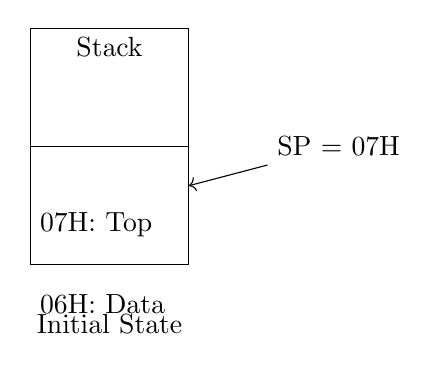
\begin{tikzpicture}[auto, node distance=2cm]
    \node [draw, rectangle, minimum width=2cm, minimum height=3cm] (Stack) {};
    \node at (Stack.north) [below] {Stack};
    
    \draw (Stack.west) -- (Stack.east);
    \node at ([yshift=-1cm]Stack.west) [right] {07H: Top};
    \node at ([yshift=-2cm]Stack.west) [right] {06H: Data};
    
    \node [right=1cm of Stack] (Info) {SP = 07H};
    \draw [->] (Info) -- ([yshift=-0.5cm]Stack.east);
    
    \node [below=0.5cm of Stack, align=center] {Initial State};
\end{tikzpicture}
\captionof{figure}{Stack Structure}
\end{center}

\begin{center}
\begin{lstlisting}[language=, caption={Stack Operation Example}]
MOV SP,#30H         ; Initialize stack pointer
PUSH ACC            ; Save accumulator
PUSH B              ; Save B register
POP B               ; Restore B register
POP ACC             ; Restore accumulator
\end{lstlisting}
\end{center}

\begin{itemize}
    \item \keyword{LIFO Structure}: Last In, First Out data organization
    \item \keyword{SP Auto-increment}: Stack pointer automatically adjusts
    \item \keyword{Subroutine Calls}: Stack saves return addresses
    \item \keyword{Register Preservation}: Save/restore register contents
\end{itemize}
\end{solutionbox}

\begin{mnemonicbox}
\mnemonic{PUSH Puts Up, Stack Holds, POP Pulls Out}
\end{mnemonicbox}

\questionmarks{5(a)}{3}{Explain branching instruction with example.}

\begin{solutionbox}
Branching instructions alter program flow based on conditions or unconditionally.

\begin{center}
\captionof{table}{Branching Instructions}
\begin{tabulary}{\linewidth}{|L|L|L|}
\hline
\textbf{Type} & \textbf{Instruction} & \textbf{Example} \\ \hline
\textbf{Unconditional} & \code{LJMP address} & \code{LJMP 2000H} \\ \hline
\textbf{Conditional} & \code{JZ address} & \code{JZ ZERO\_LABEL} \\ \hline
\textbf{Call/Return} & \code{LCALL address} & \code{LCALL SUBROUTINE} \\ \hline
\end{tabulary}
\end{center}

\begin{center}
\begin{lstlisting}[language=, caption={Branching Example}]
MOV A,#00H          ; Load zero
JZ ZERO_FOUND       ; Jump if A is zero
LJMP CONTINUE       ; Jump to continue
ZERO_FOUND:
    MOV R0,#01H     ; Set flag
CONTINUE:
    NOP             ; Continue execution
\end{lstlisting}
\end{center}

\begin{itemize}
    \item \keyword{Program Control}: Changes execution sequence
    \item \keyword{Conditional Jumps}: Based on flag register status
    \item \keyword{Address Range}: Can jump to any program memory location
\end{itemize}
\end{solutionbox}

\begin{mnemonicbox}
\mnemonic{Jump Changes Control Flow}
\end{mnemonicbox}

\questionmarks{5(b)}{4}{Interface 8 leds with microcontroller and write a program to turn on and off.}

\begin{solutionbox}
\begin{center}
\begin{tikzpicture}[auto, node distance=2cm]
    \node [gtu block, minimum height=5cm] (8051) {8051 Port 1};
    
    \foreach \i in {0,1,2,3,4,5,6,7} {
        \draw [->] ([yshift=2cm - \i*0.5cm]8051.east) -- ++(1,0) node[right, draw, circle, inner sep=1pt] (Led\i) {D} -- ++(1,0) node[right, ground] {};
        \node at ([yshift=2cm - \i*0.5cm]8051.east) [left] {P1.\i};
    }
\end{tikzpicture}
\captionof{figure}{LED Interfacing Circuit}
\end{center}

\begin{center}
\begin{lstlisting}[language=, caption={LED Blink Program}]
ORG 0000H
MAIN:
    MOV P1,#0FFH        ; Turn ON all LEDs
    CALL DELAY          ; Wait
    MOV P1,#00H         ; Turn OFF all LEDs  
    CALL DELAY          ; Wait
    SJMP MAIN           ; Repeat

DELAY:
    MOV R0,#0FFH        ; Outer loop counter
LOOP1:
    MOV R1,#0FFH        ; Inner loop counter  
LOOP2:
    DJNZ R1,LOOP2       ; Inner delay loop
    DJNZ R0,LOOP1       ; Outer delay loop
    RET                 ; Return
END
\end{lstlisting}
\end{center}

\begin{itemize}
    \item \keyword{Current Limiting}: Resistors protect LEDs from high current
    \item \keyword{Logic High}: Writing 1 to port pin turns ON LED (if wired to ground)
    \item \keyword{Delay Loop}: Nested loops create visible blink delay
\end{itemize}
\end{solutionbox}

\questionmarks{5(c)}{7}{Interface LCD with microcontroller and write a program to display "welcome".}

\begin{solutionbox}
\begin{center}
\begin{tikzpicture}[auto, node distance=2.5cm]
    \node [gtu block, minimum height=4cm] (8051) {8051};
    \node [gtu block, right=4cm of 8051, minimum height=4cm] (LCD) {16x2 LCD};
    
    % Data Lines
    \draw [->] ([yshift=1cm]8051.east) -- node[above] {P2.0-P2.3} ([yshift=1cm]LCD.west);
    \node at ([yshift=1cm]LCD.west) [right] {D4-D7};
    
    % Control Lines
    \draw [->] ([yshift=0cm]8051.east) -- node[above] {P1.0} ([yshift=0cm]LCD.west);
    \node at ([yshift=0cm]LCD.west) [right] {RS};
    
    \draw [->] ([yshift=-1cm]8051.east) -- node[above] {P1.1} ([yshift=-1cm]LCD.west);
    \node at ([yshift=-1cm]LCD.west) [right] {EN};
    
    \draw [->] (LCD.south) -- ++(0,-0.5) node[ground] {R/W (GND)};
\end{tikzpicture}
\captionof{figure}{LCD Interface Connections}
\end{center}

\begin{center}
\begin{lstlisting}[language=, caption={LCD Display Program}]
ORG 0000H
    CALL LCD_INIT       ; Initialize LCD
    CALL DISPLAY_MSG    ; Display message
    SJMP $              ; Stop here

LCD_INIT:
    MOV P2,#38H         ; Function set: 8-bit, 2-line
    CALL COMMAND
    MOV P2,#0EH         ; Display ON, Cursor ON
    CALL COMMAND  
    MOV P2,#01H         ; Clear display
    CALL COMMAND
    MOV P2,#06H         ; Entry mode set
    CALL COMMAND
    RET

DISPLAY_MSG:
    MOV DPTR,#MESSAGE   ; Point to message
NEXT_CHAR:
    CLR A
    MOVC A,@A+DPTR      ; Read character
    JZ DONE             ; If zero, end of string
    CALL SEND_CHAR      ; Send character to LCD
    INC DPTR            ; Next character
    SJMP NEXT_CHAR
DONE:
    RET

COMMAND:
    CLR P1.0            ; RS = 0 for command
    SETB P1.1           ; EN = 1
    CLR P1.1            ; EN = 0 (pulse)
    CALL DELAY
    RET

SEND_CHAR:
    MOV P2,A            ; Put character on data lines
    SETB P1.0           ; RS = 1 for data
    SETB P1.1           ; EN = 1
    CLR P1.1            ; EN = 0 (pulse)
    CALL DELAY
    RET

DELAY:
    MOV R0,#50          ; Delay routine
DELAY_LOOP:
    MOV R1,#255
DELAY_INNER:
    DJNZ R1,DELAY_INNER
    DJNZ R0,DELAY_LOOP
    RET

MESSAGE:
    DB "WELCOME",0       ; Message string with null terminator
END
\end{lstlisting}
\end{center}

\begin{center}
\captionof{table}{LCD Interface Pins}
\begin{tabulary}{\linewidth}{|L|L|L|}
\hline
\textbf{8051 Pin} & \textbf{LCD Pin} & \textbf{Function} \\ \hline
\textbf{P2.0-P2.3} & D4-D7 & 4-bit data lines \\ \hline
\textbf{P1.0} & RS & Register select (0=command, 1=data) \\ \hline
\textbf{P1.1} & EN & Enable pulse \\ \hline
\textbf{GND} & R/W & Read/Write (tied to ground for write) \\ \hline
\end{tabulary}
\end{center}

\begin{itemize}
    \item \keyword{4-bit Mode}: Uses only upper 4 data lines to save pins
    \item \keyword{Control Signals}: RS selects command/data, EN provides timing pulse
    \item \keyword{Character Display}: Each character sent as ASCII code
    \item \keyword{Initialization}: Required command sequence for proper operation
\end{itemize}
\end{solutionbox}

\begin{mnemonicbox}
\mnemonic{LCD Displays Characters with Commands and Data}
\end{mnemonicbox}

\questionmarks{5(a OR)}{3}{Explain logical instruction with example.}

\begin{solutionbox}
Logical instructions perform bitwise operations on data, useful for manipulating individual bits.

\begin{center}
\captionof{table}{Logical Instructions}
\begin{tabulary}{\linewidth}{|L|L|L|}
\hline
\textbf{Instruction} & \textbf{Example} & \textbf{Function} \\ \hline
\textbf{ANL} & \code{ANL A,\#0FH} & Bitwise AND operation \\ \hline
\textbf{ORL} & \code{ORL A,\#F0H} & Bitwise OR operation \\ \hline
\textbf{XRL} & \code{XRL A,\#FFH} & Bitwise XOR operation \\ \hline
\end{tabulary}
\end{center}

\begin{center}
\begin{lstlisting}[language=, caption={Logical Operations}]
MOV A,#55H          ; A = 01010101B
ANL A,#0FH          ; A = 00000101B (mask upper bits)
ORL A,#F0H          ; A = 11110101B (set upper bits)
XRL A,#FFH          ; A = 00001010B (complement all bits)
\end{lstlisting}
\end{center}

\begin{itemize}
    \item \keyword{Bit Manipulation}: Used for setting, clearing, and testing bits
    \item \keyword{Masking Operations}: ANL clears unwanted bits
    \item \keyword{Flag Effects}: Updates parity flag based on result
\end{itemize}
\end{solutionbox}

\begin{mnemonicbox}
\mnemonic{AND Masks, OR Sets, XOR Toggles}
\end{mnemonicbox}

\questionmarks{5(b OR)}{4}{Interface 7 segment with microcontroller.}

\begin{solutionbox}
\begin{center}
\begin{tikzpicture}[auto, node distance=2cm]
    \node [gtu block, minimum height=4cm] (8051) {8051 Port 1};
    \node [gtu block, right=3cm of 8051, minimum height=4cm, align=center] (Disp) {7-Segment\\Display};
    
    \foreach \i/\label in {0/a, 1/b, 2/c, 3/d, 4/e, 5/f, 6/g, 7/dp} {
        \draw [->] ([yshift=1.75cm - \i*0.5cm]8051.east) -- node[above, scale=0.6] {330$\Omega$} ([yshift=1.75cm - \i*0.5cm]Disp.west);
        \node at ([yshift=1.75cm - \i*0.5cm]8051.east) [left, scale=0.7] {P1.\i};
        \node at ([yshift=1.75cm - \i*0.5cm]Disp.west) [right, scale=0.7] {\label};
    }
\end{tikzpicture}
\captionof{figure}{7-Segment Interface}
\end{center}

\begin{center}
\begin{lstlisting}[language=, caption={0-9 Counter Program}]
ORG 0000H
    MOV DPTR,#DIGIT_TABLE   ; Point to lookup table
    MOV R0,#0               ; Start with digit 0

MAIN_LOOP:
    MOV A,R0                ; Get current digit
    MOVC A,@A+DPTR          ; Get 7-segment code
    MOV P1,A                ; Display on 7-segment
    CALL DELAY              ; Wait 1 second
    INC R0                  ; Next digit
    CJNE R0,#10,MAIN_LOOP   ; Check if reached 10
    MOV R0,#0               ; Reset to 0
    SJMP MAIN_LOOP          ; Repeat

DIGIT_TABLE:
    DB 3FH, 06H, 5BH, 4FH, 66H    ; 0,1,2,3,4
    DB 6DH, 7DH, 07H, 7FH, 6FH    ; 5,6,7,8,9
END
\end{lstlisting}
\end{center}

\begin{center}
\captionof{table}{7-Segment Codes}
\begin{tabulary}{\linewidth}{|L|L|L|L|}
\hline
\textbf{Digit} & \textbf{Hex Code} & \textbf{Binary} & \textbf{Segments Lit} \\ \hline
\textbf{0} & 3FH & 00111111 & a,b,c,d,e,f \\ \hline
\textbf{1} & 06H & 00000110 & b,c \\ \hline
\textbf{2} & 5BH & 01011011 & a,b,g,e,d \\ \hline
\end{tabulary}
\end{center}

\begin{itemize}
    \item \keyword{Common Cathode}: Segments light when port pin is high
    \item \keyword{Current Limiting}: Resistors prevent segment damage
    \item \keyword{Lookup Table}: Efficient storage of segment patterns
\end{itemize}
\end{solutionbox}

\begin{mnemonicbox}
\mnemonic{Seven Segments Show Digits Clearly}
\end{mnemonicbox}

\questionmarks{5(c OR)}{7}{Interface LM 35 with microcontroller and explain block diagram of temperature controller.}

\begin{solutionbox}
\begin{center}
\begin{tikzpicture}[node distance=1.5cm, auto]
    % Block Diagram
    \node [gtu block] (LM35) {LM35 Sensor};
    \node [gtu block, right=of LM35] (ADC) {ADC0804};
    \node [gtu block, right=of ADC] (Controller) {8051 Controller};
    
    \node [gtu block, above=of Controller] (Display) {Display Unit};
    \node [gtu block, below=of Controller] (Driver) {Relay Driver};
    \node [gtu block, right=of Driver] (Heater) {Heater/Fan};
    
    \path [gtu arrow] (LM35) -- (ADC);
    \path [gtu arrow] (ADC) -- (Controller);
    \path [gtu arrow] (Controller) -- (Display);
    \path [gtu arrow] (Controller) -- (Driver);
    \path [gtu arrow] (Driver) -- (Heater);
    
    \draw [gtu arrow, dashed] (Heater) |- ([yshift=-1cm]LM35.south) -- (LM35.south);
    \node at ([yshift=-0.5cm, xshift=2cm]Heater.south) {Feedback Loop};
\end{tikzpicture}
\captionof{figure}{Temperature Controller Block Diagram}
\end{center}

\begin{center}
\begin{lstlisting}[language=, caption={Temperature Control Program}]
ORG 0000H
MAIN:
    CALL READ_TEMP      ; Read temperature from ADC
    CALL DISPLAY_TEMP   ; Show temperature on display
    CALL TEMP_CONTROL   ; Control heating/cooling
    CALL DELAY          ; Wait before next reading
    SJMP MAIN

READ_TEMP:
    CLR P2.0            ; Start ADC conversion
    SETB P2.0           ; Pulse to start
    JNB P2.1,$          ; Wait for conversion complete
    MOV A,P1            ; Read temperature data
    RET

TEMP_CONTROL:
    CJNE A,#30,CHECK_HIGH   ; Compare with setpoint (30C)
CHECK_HIGH:
    JC TEMP_LOW             ; If A < 30, temperature is low
    SETB P3.0               ; Turn ON cooling (fan)
    CLR P3.1                ; Turn OFF heating
    RET
TEMP_LOW:
    CLR P3.0                ; Turn OFF cooling
    SETB P3.1               ; Turn ON heating
    RET
END
\end{lstlisting}
\end{center}

\begin{center}
\captionof{table}{System Components}
\begin{tabulary}{\linewidth}{|L|L|}
\hline
\textbf{Component} & \textbf{Function} \\ \hline
\textbf{LM35} & Temperature sensor (10mV/$^\circ$C) \\ \hline
\textbf{ADC0804} & Analog to digital converter \\ \hline
\textbf{8051} & Main controller \\ \hline
\textbf{Relay} & Switch high power loads \\ \hline
\textbf{Display} & Show current temperature \\ \hline
\end{tabulary}
\end{center}

\begin{itemize}
    \item \keyword{Temperature Sensing}: LM35 provides 10mV per degree Celsius
    \item \keyword{ADC Conversion}: Converts analog voltage to digital value
    \item \keyword{Control Logic}: Compares with setpoint and controls relay
    \item \keyword{Feedback System}: Continuous monitoring and adjustment
\end{itemize}
\end{solutionbox}

\begin{mnemonicbox}
\mnemonic{Sense, Convert, Compare, Control Temperature Automatically}
\end{mnemonicbox}

\end{document}
